\documentclass[12pt]{article}
\usepackage{graphicx}
\usepackage[a4paper, left = 2cm, right = 2cm, top = 2cm, bottom = 2cm]{geometry}
\usepackage{listings}
\usepackage{amssymb}
\usepackage{pgfplots} 
\usepackage{amsmath}
\usepackage{hyperref}
\usepackage{url}
\usepackage{subfig}
\usepackage{algorithm}
\usepackage{algpseudocode}
\usepackage{centernot}

\newtheorem{definition}{Definition}
\newtheorem{example}{Exmaple}
\newtheorem{property}{Property}
\newtheorem{proof}{Proof}
\newcommand{\norm}[1]{\lVert#1\rVert}
\newcommand{\abs}[1]{\lvert#1\rvert}

\begin{document}
	
	\begin{titlepage}
		
		\title{Project of Parallel and Distributed Systems\\Paradigms and Models \\\vspace{1cm}
		Parallel Iterative Jacobi Method}
		\author{Student: Diego Arcelli\\ Student ID: 647979 \\
			Professor: Marco  Danelutto}
		\date{Academic Year 2021-2022}
		\maketitle
		\centering
		
\includegraphics[width=10cm]{./images/unipi_logo.png}
		
	\end{titlepage}
	
	\tableofcontents
	\newpage
	
	\section{Analysis of the problem}
	Notation premise: with $x_i^{(k)}$ we indicate the $i$-th entry of vector $x$ at iteration $k$. The pseudo-code to execute the Jacobi method sequentially, for a fixed amount of iterations, is shown in \ref{alg:seq}. Note that we are forced to use an auxiliary vector $x^\prime$ to compute the updated elements of $x$ for the current iteration, and then, before starting the following iteration, we copy the elements of $x^\prime$ in $x$. This is necessary because if at iteration $k$ we compute $x^{(k)}_1$ modifying $x$ in-place, then when we'll compute $x^{(k)}_2$, instead of using $x^{(k-1)}_1$, we'll use $x^{(k)}_1$.\\
	The $swap$ function used to copy the elements of $x^\prime$ in $x$, can be implemented in $O(1)$ time complexity, by swapping the pointers of the two arrays.
	\begin{algorithm}[H]
		\caption{Sequential code for Jacobi method}\label{alg:seq}
		\begin{algorithmic}[1]
			\Require $A$ strictly diagonally dominant matrix, $b$ vector, $limit$ positive integer
			\For{$k \gets 1$ to $limit$}
			\For{$i \gets 0 $ to $n-1$}
			\State{$x^\prime[i] \gets 0$}
			\For{$j \gets 0 $ to $n-1$}
			\If{$j \ne i$}
			\State{$x^\prime[i]  \gets x^\prime[i] - A[i,j]* x[j]$}
			\EndIf
			\EndFor
			\State{$x^\prime[i] \gets (x^\prime[i] + b[i])/A[i,i]$}
			\EndFor
			\State{swap($x$, $x^\prime$)}
			\EndFor
		\end{algorithmic}
	\end{algorithm}
	\noindent Let's now analyze how we can exploit the properties of the algorithm in order to parallelize it. The first important thing we notice is that in order to compute the updated values for the vector $x$ at iteration $k$, we need the full updated vector $x$ at iteration $k-1$, therefore the iterations of the algorithm need to be strictly sequential.\\
	A relevant property of the algorithm that we can notice from the pseudo-code, is that each element of the vector $x^{(k)}$ is computed independently from the others elements, since in order to to compute $x_i^{(k)}$ we just need the old vector $x^{(k-1)}$ and the matrix $A$. Therefore the iterations of the loop at line 2 of the pseudo-code, can be executed in parallel, which is the classical application of a map pattern. So, if we have $nw$ workers available, we can assign to each worker a partition of indices of $x$ to compute.\\
	The innermost loop at line 4 is used to compute a sum of $n-1$ elements, which is the classical application of a reduce pattern. This is done inside the loop that we already said we can parallelize using a map pattern, so if we want to implement also the reduce, for each one of the $nw$ workers of the map, we have to arrange other $nw^\prime$ additional workers that can be used to compute in parallel the summation.\\
	The introduction of a reduce inside each map would increase the overhead, since each worker assigned to the map would have to coordinate its computations with the workers that it uses for the reduce. Moreover, if the additional $nw\cdot nw^\prime$ workers arranged for the reduce, are just used to increase the parallel degree of the map, we would obtain the same theoretical speedup (this is shown in the time analysis section) but which much less overhead. Therefore I decided to do not implement the reduce.\\
	Even if we only implement the map, there some synchronization problems that we need to care about:
	\begin{enumerate}
		\item Start iteration $k+1$ only after all the workers finished their computations for iteration $k$, since the iterations must be strictly sequential 
		\item Executing the swap of the main and auxiliary vectors only after all the workers finished their computations for the current iteration, otherwise it might happen that the vectors are swapped while some workers are still computing their portion of $x^{(k)}$
		\item Keep track of the number of iterations so that all the workers will stop after $limit$ iterations
	\end{enumerate}
	The first problem can be solved simply by putting a barrier after the execution of the map, so that all the workers will be forced to wait the others before starting the next iteration. In this way we can also solve the third problem by selecting one of the worker to count the number of iterations of the algorithm executed so far. The designated worker can simply use a shared variable among the workers, that it will increase by one before the barrier. Since the variable is modified by just one worker it doesn't need synchronization mechanism to be accessed, even if it is shared. This solution guarantees that before starting iteration $k$ the shared variable will have value $k$ for all the workers, so that every worker can individually check if $k = limit$ and stop its execution if it is the case. To solve the second problem we need to introduce a second barrier, which has to be placed between the end of the map an the previously defined next iteration barrier. Between this new defined barrier and the next iteration barrier, one of the workers will be selected to execute the swap (it can be the same one that counts the iterations). In this way the swap will happen only after every worker finished its computations for the current iteration and before starting the next iteration.\\
	The pseudo-code of the routine executed by a worker is showed in \ref{alg:par}.
	\begin{algorithm}[H]
		\caption{Worker pseudo-code}\label{alg:par}
		\begin{algorithmic}[1]
			\Require $A$ strictly diagonally dominant matrix, $b$ vector, $limit$ positive integer
			\While{$k < limit$}
			\For{$i \gets start $ to $end$}
			\State{$x^\prime[i] \gets 0$}
			\For{$j \gets 0 $ to $n-1$}
			\If{$j \ne i$}
			\State{$x^\prime[i] \gets x^\prime[i] - A[i,j]* x[j]$}
			\EndIf
			\EndFor
			\State{$x^\prime[i] \gets (x^\prime[i] + b[i])/A[i,i]$}
			\EndFor
			\State{\textbf{Vectors swap barrier}}
			\If{start = 0}
			\State{swap($x$, $x^\prime$)}
			\State{$k \gets k+1$}
			\EndIf
			\State{\textbf{Next iteration barrier}}
			\EndWhile
		\end{algorithmic}
	\end{algorithm}
	\noindent The variables $start$ and $end$ represent respectively the first and the last index of $x$ assigned to the worker. The worker that will update the iterations counter and execute the swap of the vectors is the one assigned to the leftmost chunk (the one with $start = 0$). Note that both of the barriers are needed because if we only use the copy barrier, it could happen that some of the workers might start the next iteration before the designated worker could swap the vectors and update the iteration counter.
	
	
	\section{Time analysis}
	In the sequential case, the time required to execute the algorithm is:
	\[ T_{seq} = T_{init} + k\Big(n^2T_\oplus + T_{swap}\Big) \]
	where $k$ is the number of iterations, $n$ is the number of rows and columns of the matrix, $T_{init}$ is the time required to initialize the computations, $T_\oplus$ is the time required to compute the expression at line 6 of \ref{alg:seq} and $T_{swap}$ is the time required to perform the swap of the vectors. $T_{init}$ includes the declaration of some variable and the creation of the auxiliary array. If we consider negligible the initialization and the swap times, then the execution time is more or less: 
	\[ T_{seq} \approx kn^2T_\oplus \]
	In the parallel case, the loop at line 2 of \ref{alg:seq} is parallelized, so, with $nw$ workers available, the program will execute at the same time $nw$ parallel loops, each of which will iterate more or less $\frac{n}{nw}$ times. The overhead introduced is given by the creation and the termination of the workers, by the time required to compute and assign tasks to the workers and by the time required to manage the barriers, so overall that the parallel time is:
	\[T_{par}(nw) = T_{init} + T_{split} + T_{spawn} + k\Big(\frac{n}{nw}nT_\oplus + T_{synch} + T_{swap} + T_{synch}\Big) + T_{stop} \]
	where $T_{spawn}$ and $T_{stop}$ are the times required to spawn and terminate the workers, $T_{split}$ is the time required to compute and split the tasks among the workers and $T_{synch}$ is the time required to handle the barrier. Again, if we consider negligible the times required for the preparations, the synchronization and the swap, then the parallel time is approximately:
	\[T_{par}(n) \approx k\frac{n}{nw}nT_\oplus \]
	If we had decided to implement the reduce too, assigning $nw_1$ workers to the map and $nw_2$ workers to each worker of the map for the reduce, then the parallel time would have changed as follows:
	\[ T^\prime_{par}(nw) \approx k\Big[\frac{n}{nw_1}\Big(\frac{n}{nw_2}T_\oplus + nw_2T_\oplus \Big) \Big] = k\frac{n}{nw_1}\frac{n}{nw_2}T_\oplus + knw_2T_\oplus \approx k\frac{n}{nw_1}\frac{n}{nw_2}T_\oplus \]
	since for each map we could have computed in parallel $nw_2$ partial sums of $\frac{n}{nw_2}$ elements each, and then we would have computed the final sum summing up the $nw_2$ partial sums. If in $T_{par}$ we set $nw = nw_1\cdot nw_2$, then the time is the same of $T^\prime_{par}$. Actually if we don't exclude from $T^\prime_{par}$ the time needed to compute the partial sums, we also have the term $k nw_2T_\oplus$, and so $T_{par}$ is even better than $T^\prime_{par}$. From this analysis we draw the conclusion that if we only implement the map, with the same resources we get an even better theoretical execution time than implementing both the map and the reduce. Furthermore the implementations of the reduce would introduce overheads and more synchronization problems that are not present if we only implement the map.\\
	The speedup we can achieve is:
	\[ Speedup(nw) = \frac{T_{init} + k\Big(n^2T_\oplus + T_{swap}\Big)}{T_{init} + T_{split} + T_{spawn} + k\Big(\frac{n}{nw}nT_\oplus + T_{synch} + T_{swap} + T_{synch}\Big) + T_{stop}}\]
	If we exclude the negligible times then we get:
	\[ Speedup(nw) \approx \frac{kn^2t_\oplus}{k\frac{n}{nw}nt_\oplus} = nw\]
	which is the ideal speedup which we can theoretically obtain with a map pattern. Of course to have a better estimate of the speedup we should consider the serial fraction of the program. We can make a rough estimation by considering that the total number of operations done by the algorithm is more or less in the order of $kn^2$. since we have to do some fixed amount of operations inside the three loops. Ideally, With $n$ workers, every worker could compute its own $x_i^{(k)}$ in more or less $n$ operations, reducing the number of operations to $kn$. Therefore a rough estimation of the serial fraction is:
	\[ f = \frac{kn}{kn^2} = \frac{1}{n}\]
	if we now consider the speedup given by the Amdahl's law, we have that in the best case the maximum speedup is:
	\[ Speedup < \frac{1}{f} = \frac{1}{\frac{1}{n}} = n\]
	So the speedup is upper-bounded by the number of rows/columns of the matrix. This makes sense, since in an ideal scenario, we would have a worker for each component of the vector $x$, reducing the cost of a single iteration of the algorithm from $O(n^2)$ to $O(n)$.
	
	\section{Implementation details}
	The parallel program has been implemented in three versions:
	\begin{itemize}
		\item[--] The first using native C++ threads 
		\item[--] The second using FastFlow
		\item[--] The third using OpenMP
	\end{itemize}
	The program has been implemented defining a class called \verb|Jacobi| which has as attributes the coefficients matrix $A$, the vector $b$ and an integer $n$ that represent the size of $A$ and $b$. For each implementation of the algorithm (the sequential and the three parallel ones) there's a corresponding method to solve the linear system $Ax = b$, using that specific implementation, by providing as parameters the number of iterations of the algorithm and the number of workers (for the parallel versions). For all the implementations the solution vector $x$ is initialized setting all the elements to 0, and to assure that algorithm will converge, $A$ it's generated randomly to be strictly diagonally dominant. 
	\subsection{C++ threads}
	In the implementation with native C++ threads I used the fork-join mechanism to spawn $nw$ threads, each of them is assigned to a contiguous chunk of $x$ of size $\lfloor\frac{n}{nw}\rfloor$ according to the following procedure:
	\begin{algorithmic}
		\State $\Delta \gets \lfloor\frac{n}{nw}\rfloor$
		\For{$i \gets 0$ to  $nw$}
			\State $start_i \gets i*\Delta$
			\State $end_i \gets start_i + \Delta - 1$
		\EndFor
		\State $end_{nw} \gets n-1$
	\end{algorithmic}
	Then each thread will execute code identical to the one in \ref{alg:par}. For the implementation of the barrier I used the \verb*|barrier| class introduced in C++20.
	\subsection{FastFlow}
	For the FastFlow implementation I used the \verb|ParalleFor| class to parallelize the loop at line 2 of \ref{alg:seq}. An object of class \verb|ParalleFor| is created before starting the algorithm, in order to prepare the $nw$ workers in advance, and then we call the \verb*|parallel_for| method inside the main loop of of the algorithm. The function passed to the parallel \verb*|parallel_for| method is the following:
	\begin{algorithmic}
		\Function{parallel\_for\_iteration}{$i$}
		\State $x^\prime[i] \gets 0$
		\For{$j \gets 0$ to  $n-1$}
		\If{$i \ne j$}
		\State $x^\prime[i] \gets x^\prime[i] - A[i,j]*x[j]$
		\EndIf
		\EndFor
		\State $x^\prime[i] \gets (x^\prime[i] + b[i])/A[i,i]$
		\EndFunction
	\end{algorithmic}
	After the call of the parallel for method, the counter of the loop is increased and the vectors are swapped, and this is done sequentially by the main thread of the program. Note that we do not need to explicitly define the barrier since the call of the \verb*|parallel_for| method is an implicit barrier for the workers. 
	\subsection{OpenMP}
	For the OpenMP implementation I simply parallelized the second innermost loop at line 2 of algorithm \ref{alg:seq}, using the \verb|#pragama omp parallel for| directive, using the static scheduling that divides the loop in $nw$ chunks of equal size. Like in the case of FastFlow, the end of the parallelized for is an implicit barrier for the threads, so we do not need to define the barrier explicitly.  
	\section{Manual}
	The source code, the scripts written for the experiments and a detailed manual of the program are available at \href{https://github.com/DiegoArcelli/Parallel-And-Distributed-Systems-Project}{this} repository.\\ 
	To compile the code is sufficient to execute the command \verb*|make| in the \verb*|src| directory of the project. The compilation will produce the executable \verb*|main| which can be launched to execute the program, providing the following arguments:
	\begin{itemize}
		\item[--] \verb|n|: the number of rows and columns of the matrix
		\item[--] \verb|nw|: the number of workers that will be used in the parallel versions of the algorithm
		\item[--] \verb|iters|: the number of iterations of the algorithm
		\item[--] \verb|mode|: an integer number which specifies which implementations of the algorithm will be executed
	\end{itemize} 
	The possible values of \verb|mode|, with the corresponding effects, can be showed by launching the program with no argument. Once executed the program will run the versions of the algorithm required (according to the value of \verb|mode|), and it will print their execution times. 
	
	\section{Experiments}
	The main goals of the experiments that we will execute are the following: 
	\begin{itemize}
		\item[--] Comparing the performances obtained by the three implementations 
		\item[--] Check how the performances change with respect to the size of the matrix
		\item[--] Comparing the actual performances to the ideal ones
	\end{itemize}
	To compare the performances of the three implementations we'll measure the times obtained when executing the algorithm with $nw$ workers, varying $nw$ from 1 to 32. Then from the times we'll derive the speedup and the efficiency of the three implementations. To see if the size of the matrix impacts on the performances, we'll repeat this procedure twice, first on 1000$\times$1000 matrix and then on a 10000$\times$10000 matrix.\\
	After that we'll execute the algorithms with a fixed number of workers on matrices of different sizes, to better understand the impact that the size of the matrix has on the performances.\\
	The times are measured defining a \verb*|timer| class which uses the RAII mechanism to get the creation and the destruction time of its instances, as we saw during the lectures. The times reported include the allocation and the de-allocation of the auxiliary vector, but not the creation and the initialization of the main vector $x$, which is created and initialized in advance, by setting all the elements to 0. For all the experiments the number of iterations of the algorithm has been fixed to 100.
		
	\begin{figure}[H]
		\centering
		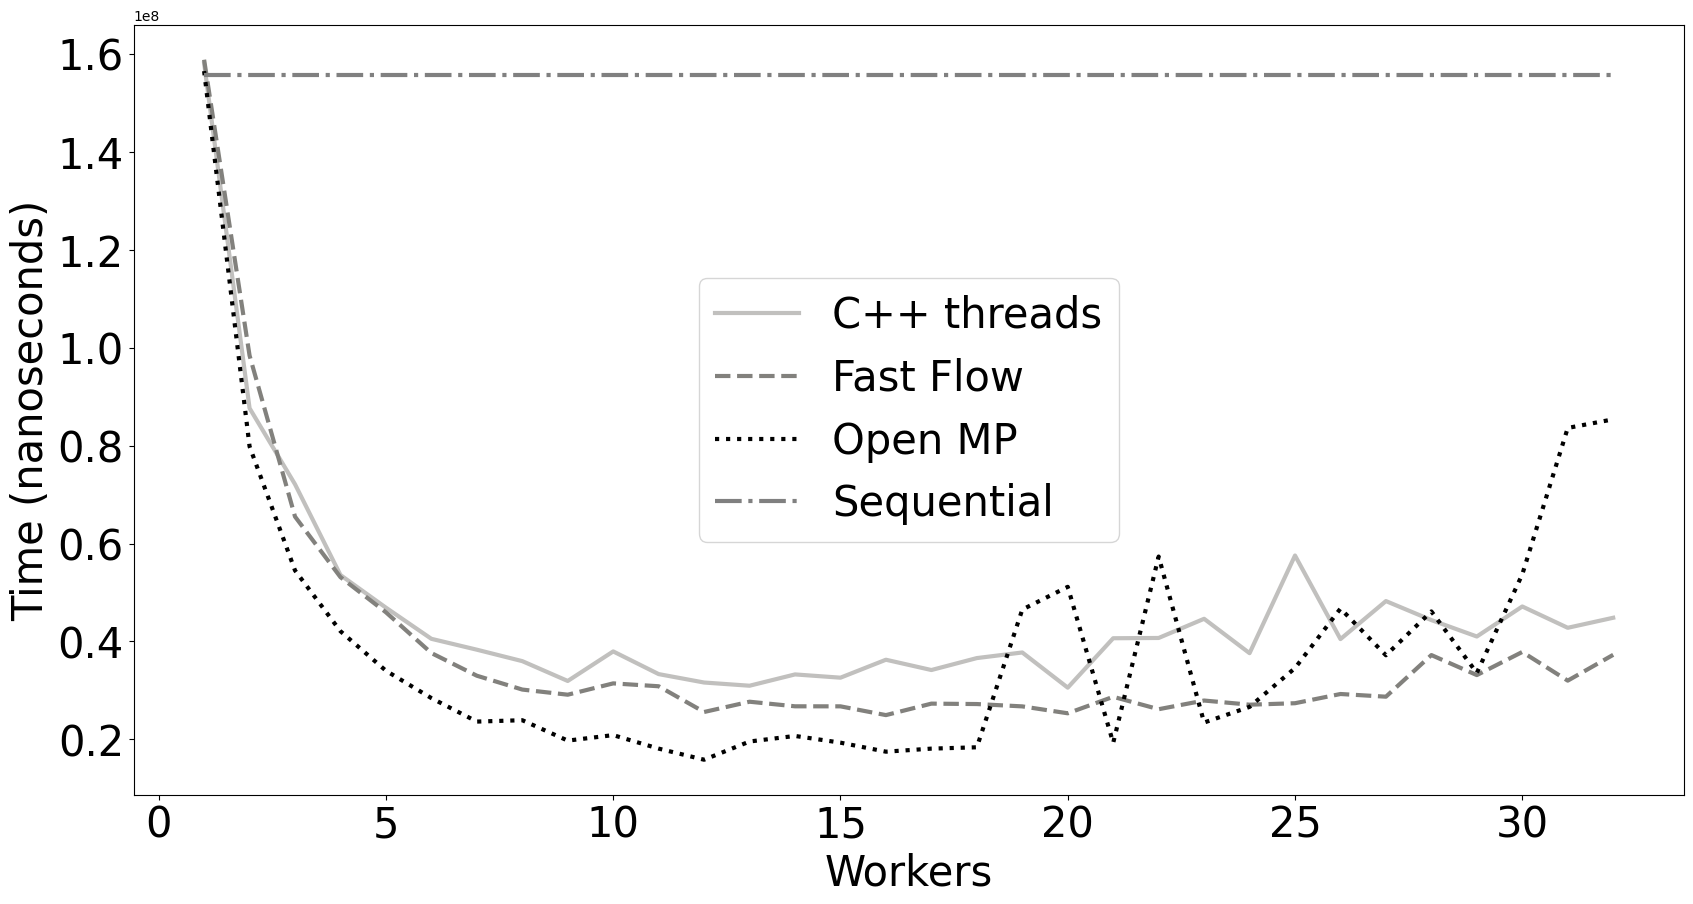
\includegraphics[width=13cm]{./images/time_vs_cores_1000}
		\caption{Time vs workers for matrix size 1000}
	\end{figure}
	
	\begin{figure}[H]
		\centering
		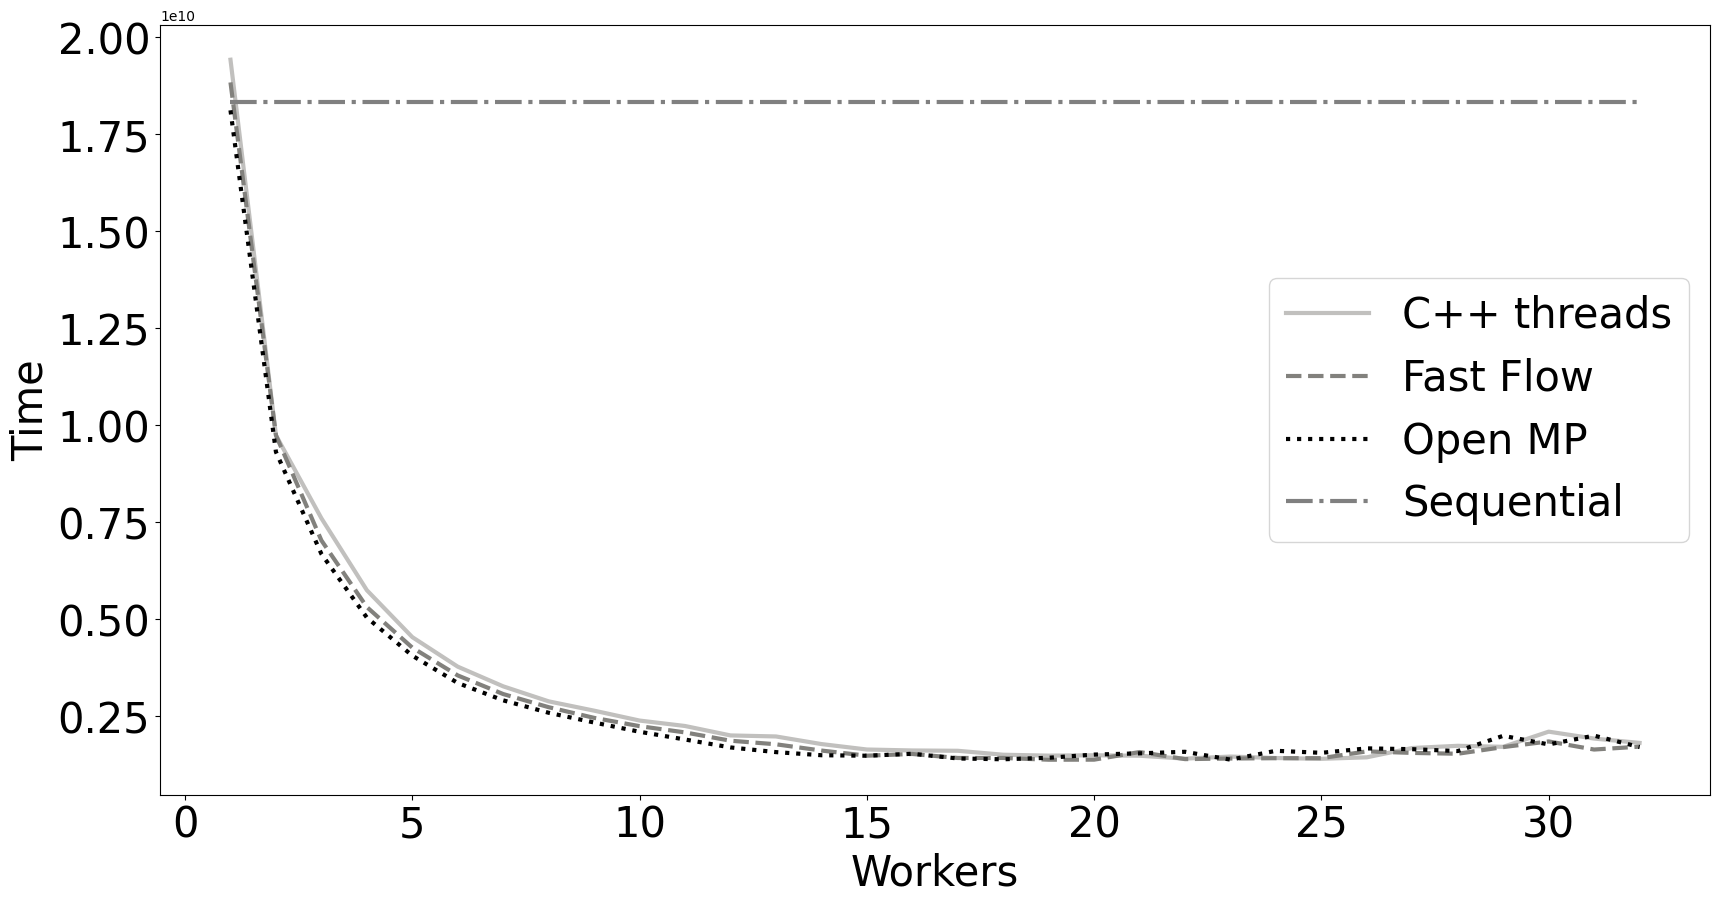
\includegraphics[width=13cm]{./images/time_vs_cores_10000}
		\caption{Time vs workers for matrix size 10000}
	\end{figure}

	\begin{figure}[H]
		\centering
		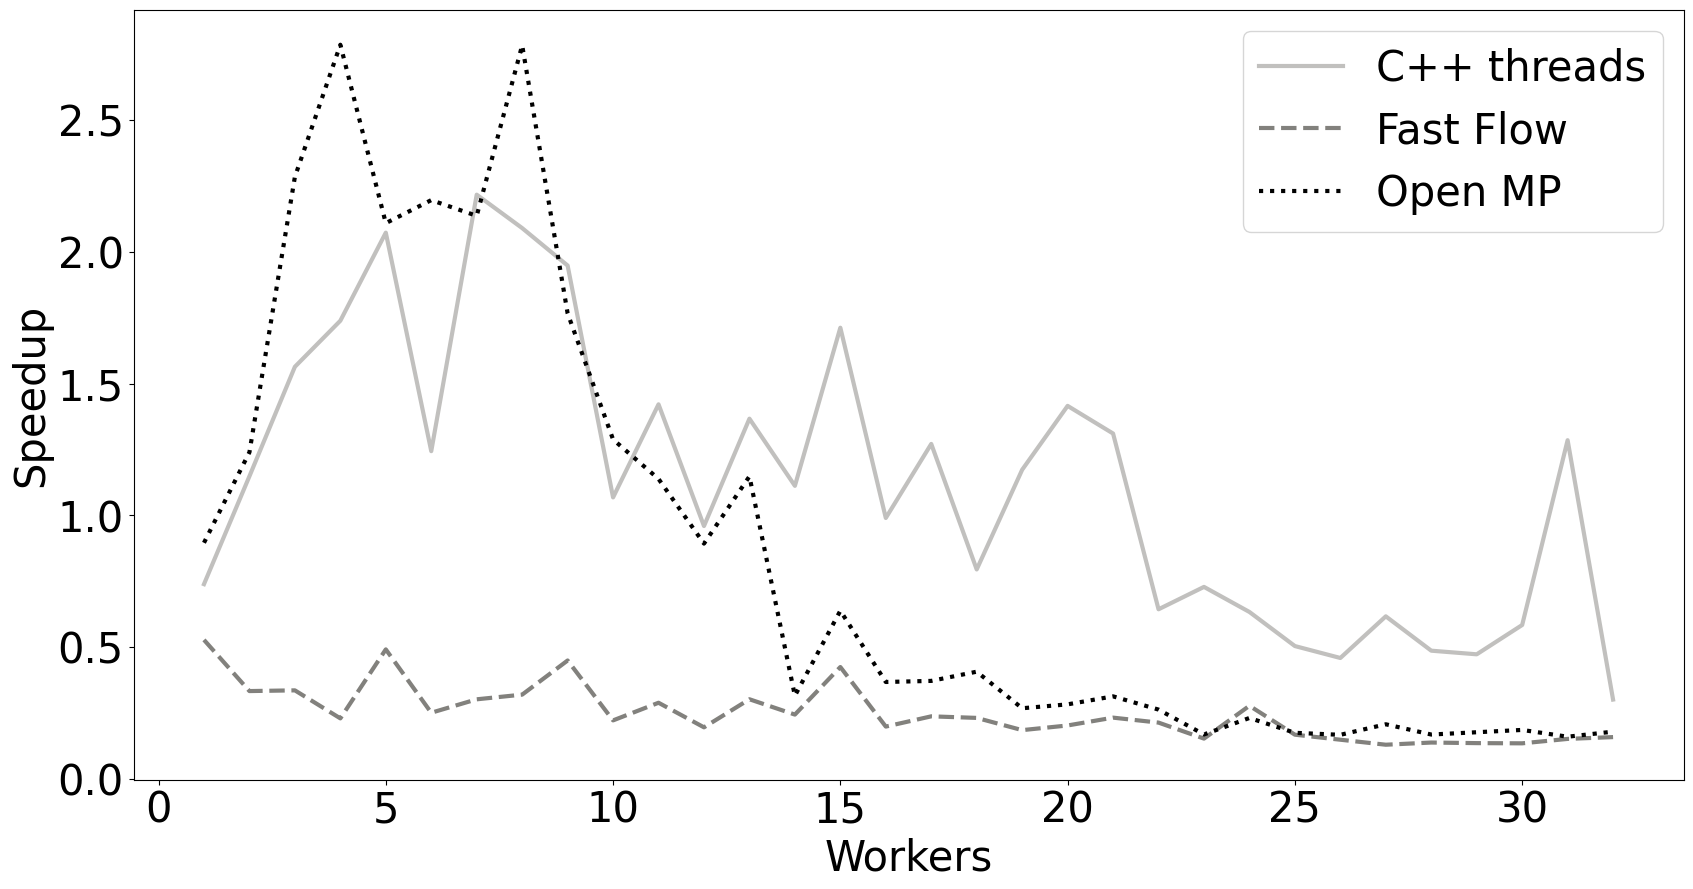
\includegraphics[width=13cm]{./images/speedup_vs_cores_1000}
		\caption{Speedup vs workers for matrix size 1000}
	\end{figure}

	\begin{figure}[H]
		\centering
		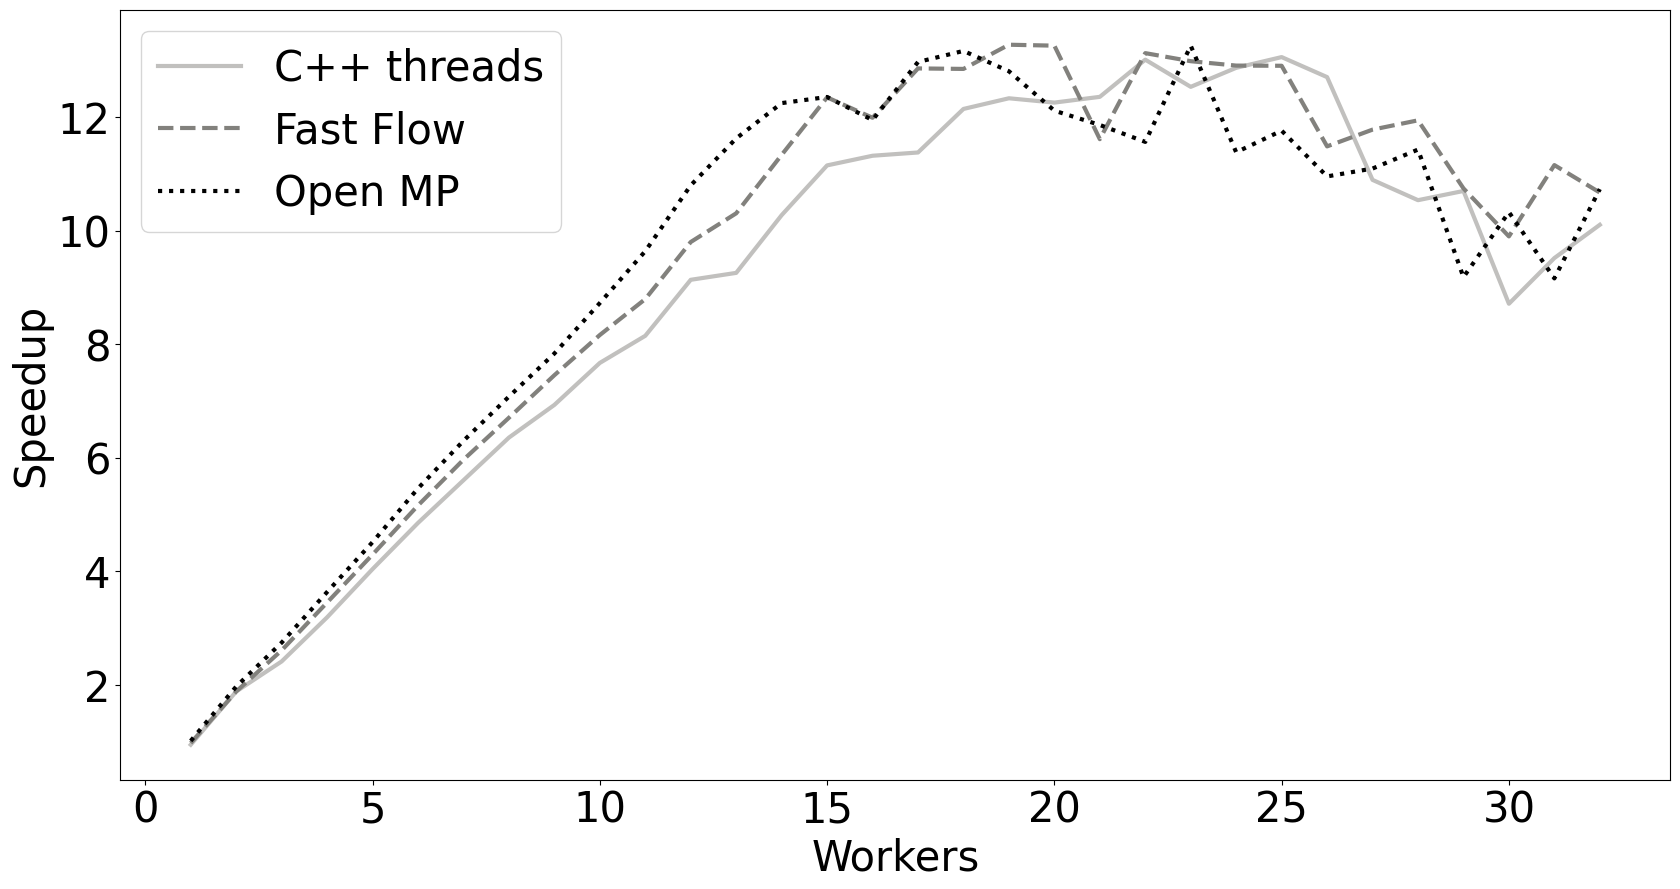
\includegraphics[width=13cm]{./images/speedup_vs_cores_10000}
		\caption{Speedup vs workers for matrix size 10000}
	\end{figure}

	\begin{figure}[H]
		\centering
		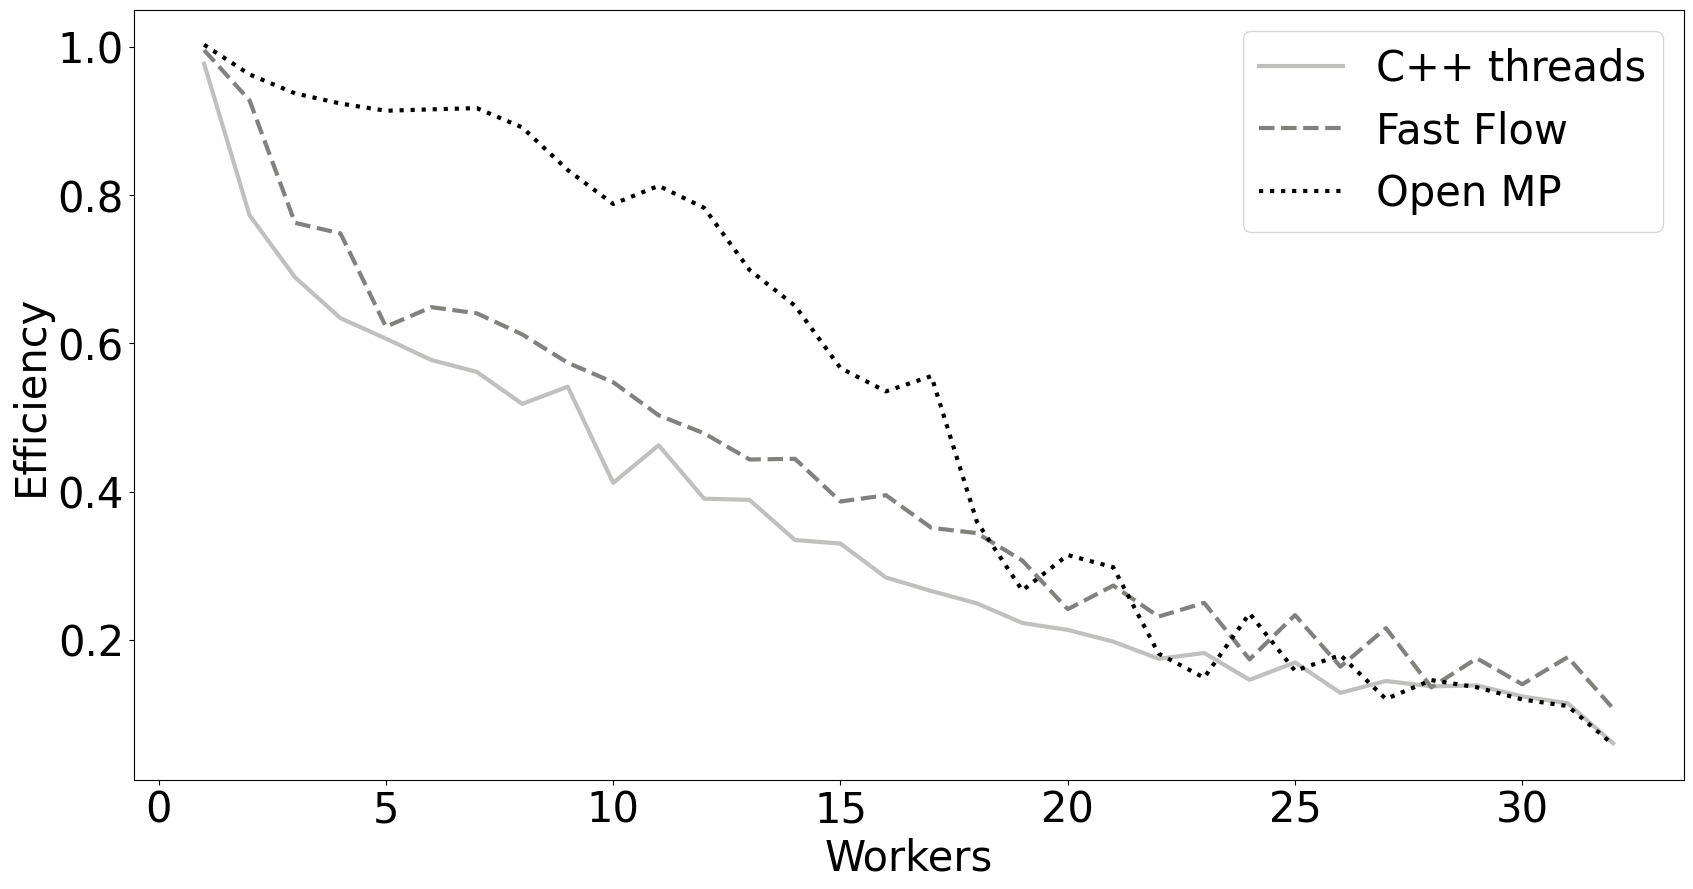
\includegraphics[width=13cm]{./images/efficiency_vs_cores_1000}
		\caption{Efficiency vs workers for matrix size 1000}
	\end{figure}

	\begin{figure}[H]
		\centering
		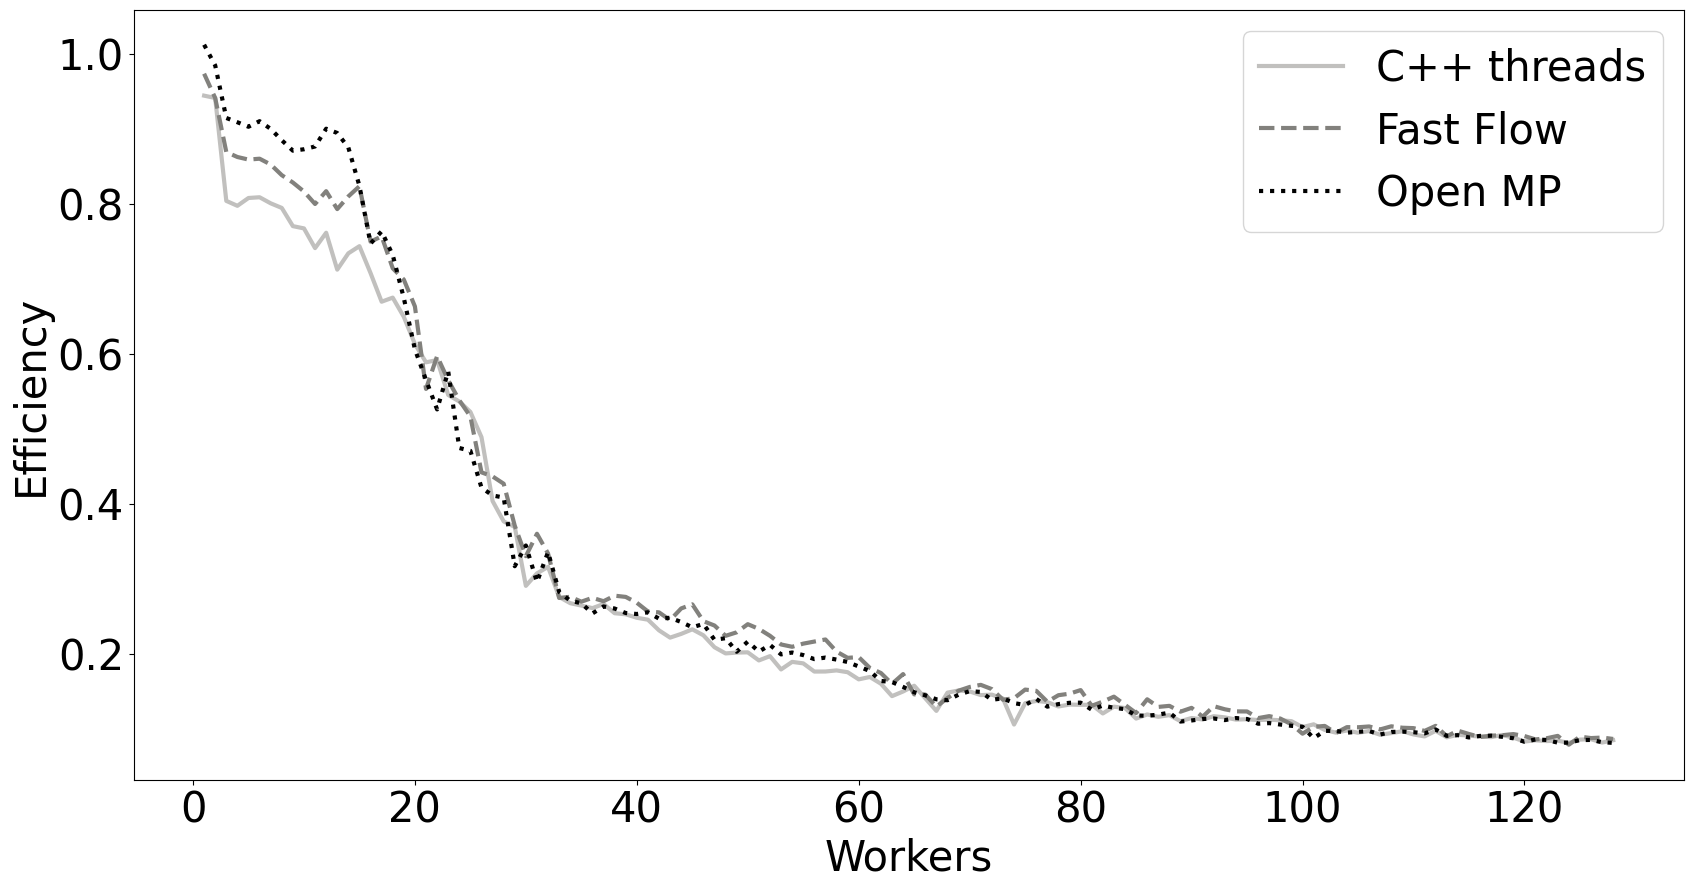
\includegraphics[width=13cm]{./images/efficiency_vs_cores_10000}
		\caption{Efficiency vs workers for matrix size 10000}
	\end{figure}

	\begin{figure}[H]
		\centering
		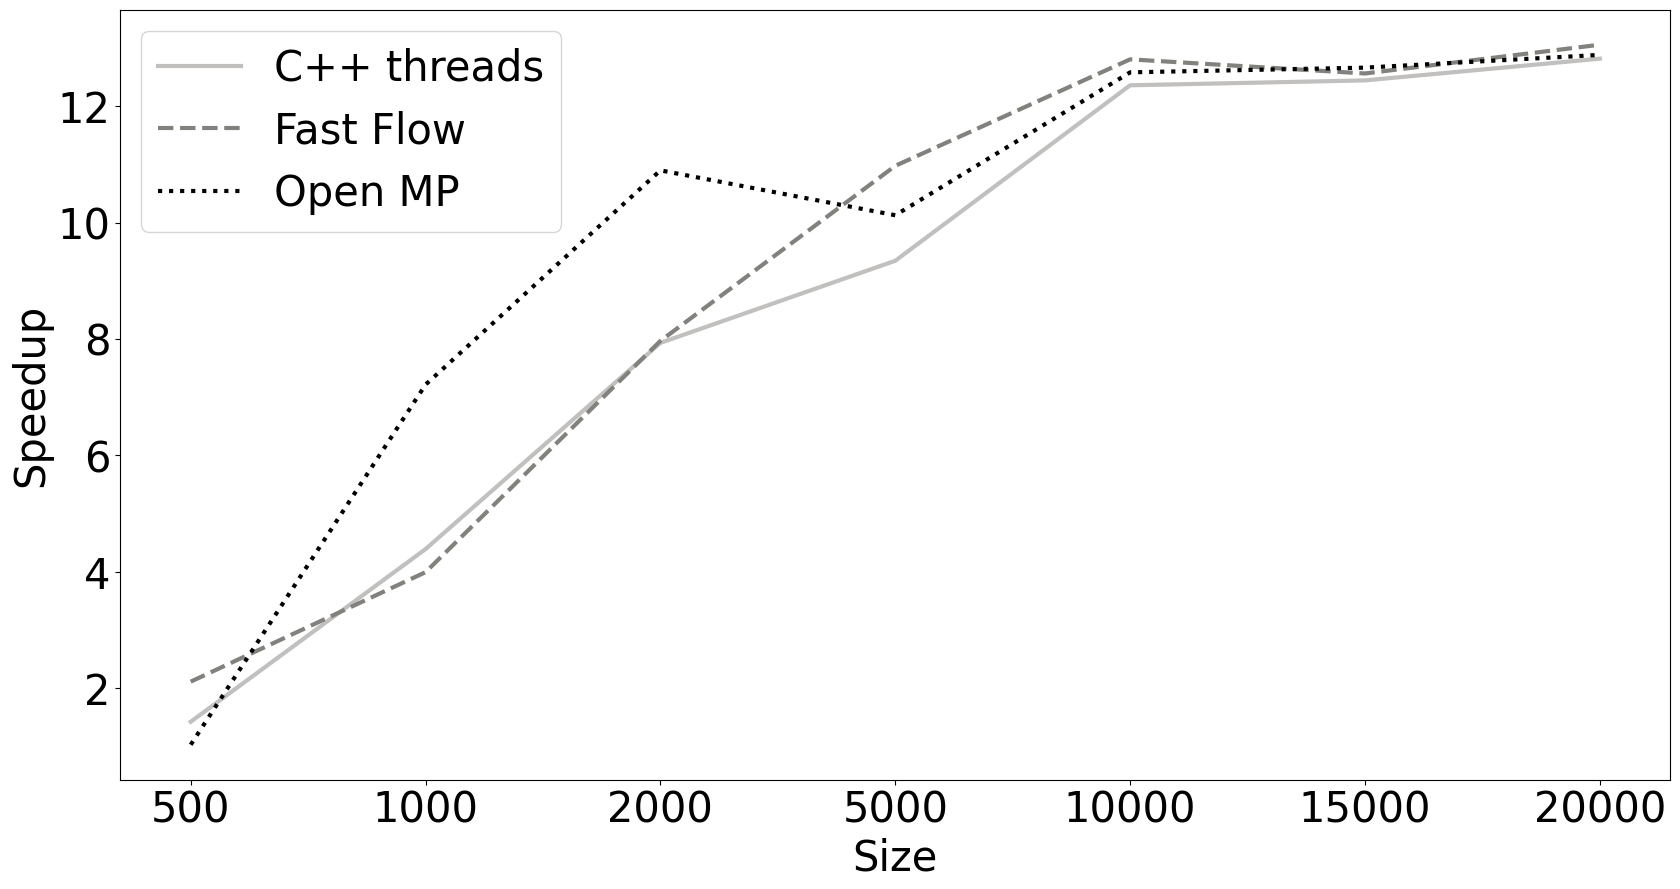
\includegraphics[width=13cm]{./images/speedup_vs_size}
		\caption{Speedup vs matrix size with 16 workers}
		\label{fig:speed_vs_size}
	\end{figure}


	\section{Conclusions}
	The first thing that we notice from the experiments is that the performances get better as the dimension of the matrix increases. The speedups reached when $n$ is large are better than those reached when $n$ is small, and because of this, the efficiency decreases slower when $n$ is large. This is also confirmed from figure \ref{fig:speed_vs_size}, where we can see that the speedups increase with the size of the matrix, even though they stabilize for matrices of sizes 10000, 15000 and 20000. Maybe it would have been interesting trying with even larger matrices, but I couldn't since for matrices of larger sizes the remote machine kills the process (I presume because it allocates too much memory). The reason for which the speedup is better for large values of $n$ is probably due to the fact that with $n$ also the grain of the computations of a single worker increases, since the size of the chunk that it has to compute gets larger, and the times required for the preparation and the synchronization occupy a smaller fraction of the total execution time. Conversely when $n$ is small the fraction of time required for preparation and synchronization it's larger, and therefore the speedup is lower.\\
	In the case of $n = 1000$, the OpenMP implementation tends to do much better then the other two, and FastFlow does better than the native C++ threads implementation. For the experiments with $n = 10000$ the performances of the three implementations are very similar, even if also in this case the OpenMP versions does a little bit better than the other two, and FastFlow does a little bit better of the native C++ threads implementation. The fact that the C++ threads implementation is the worst might be caused by the fact that the threads during the execution of the program have to go through two barriers instead of one, since in the case of OpenMP and FastFlow, there's only one implicit barrier after which the control is given back to the main thread of the program, which updates the iterations counter and swap the pointers.\\
	From the plots we can see that, at least of the experiments with $n = 10000$, the the speedups tends to be close to the linear one when the number of workers is small (especially for OpenMP). As the number of workers increases, the efficiency tends to decrease, and therefore the speedup gets far from the linear one. A possible cause of this is the fact that with few workers the grain of the computations is larger, since we have to handle less threads, and each thread has to do more computations, therefore the fraction of time required for the preparation and the synchronization times, is smaller when the number of worker is small, hence we can have a better speedup. Since the speedup increases with $n$, maybe with larger values of $n$, even with an higher number of workers the speedup would have remained close to the linear one, but for the reason explained before I couldn't test this hypothesis.
	
\end{document}